\chapter{State of the Art in Optimal V2G Management}
\vspace*{2cm} % spazio verticale prima della citazione

\begin{center}
  \begin{minipage}{0.85\textwidth}
    \begin{displayquote}
      \large\itshape
      ``The green transition is the most ambitious industrial transformation ever. 
      The region of the world that develops clean technologies first will come out on top — 
      and I want it to be Europe.''
    \end{displayquote}
  \end{minipage}
\end{center}

\vspace{0.5cm}

\begin{flushright}
  --- \textsc{Ursula von der Leyen}
\end{flushright}

\section{The V2G Imperative: A Foundation of Europe's Green Transition}


Europe finds itself at the confluence of two unprecedented and deeply interlinked transformations that are reshaping the continent’s technological, economic, and societal landscape: on one hand, the large-scale electrification of the transport sector, which involves a radical shift from internal combustion engines to battery electric and hydrogen-powered vehicles, and on the other hand, a comprehensive restructuring of energy systems, encompassing the integration of renewable generation, the modernization of grids, and the deployment of advanced storage and demand-side management solutions.
\noindent
\\
These transformations are not merely aspirational targets but constitute binding legal obligations established under the \textbf{European Green Deal}, which sets the overarching climate and sustainability strategy for the European Union, and the detailed \textbf{"Fit for 55"} legislative package, which translates these ambitions into enforceable measures aimed at reducing greenhouse gas emissions by 55\% by 2030 across multiple sectors \footcite{european_commission_2021_fit_for_55}.
 The policy architecture demands a 55\% reduction in net greenhouse gas emissions by 2030, necessitating the rapid elimination of internal combustion engines alongside a dramatic expansion of renewable energy capacity, as outlined in the revised \textbf{Renewable Energy Directive }(RED III). Electric Vehicles (EVs) occupy a central position in this transition, simultaneously driving decarbonisation efforts while presenting complex challenges for grid stability and management.
\noindent

\begin{figure}[H]
    \centering
    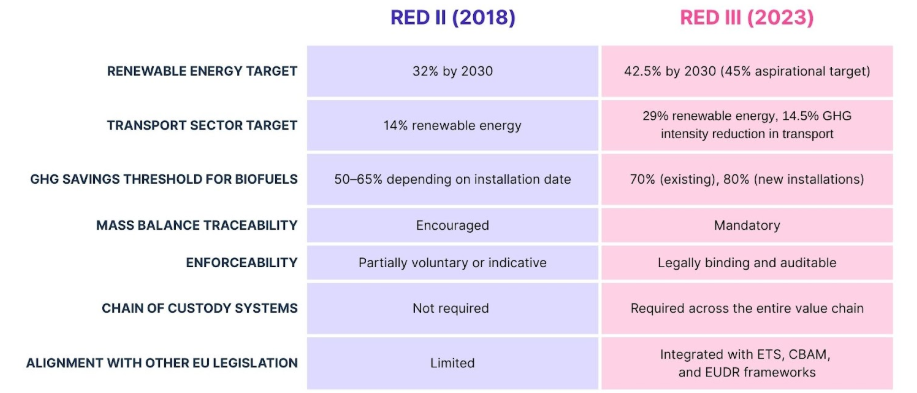
\includegraphics[width=1\linewidth]{red.png}
    \caption{RED 3}
    \label{fig:placeholder}
\end{figure}
\noindent
The initial response to mass EV adoption was characterised by considerable concern within the power sector. The prospect of millions of new electric vehicles was perceived primarily through the lens of risk—vast, temporally correlated loads threatening to overwhelm local distribution networks during peak evening hours. This perspective has undergone a fundamental reassessment. EVs are now recognised not as burdens to be managed, but as essential infrastructure for achieving Europe's energy transition objectives. 
\\
This conceptual shift finds its most concrete expression in \textbf{Vehicle-to-Grid (V2G)} technology, which fundamentally reimagines the role of electric vehicles within the energy system.
\noindent
V2G technology transforms what were previously passive, unidirectional energy consumers into active, distributed, and smart grid resources. The underlying opportunity is both elegant and substantial: private vehicles spend approximately 96\% of their operational lifetime parked and connected \footcite{evertsson2024investigating}, representing an enormous, geographically distributed, and currently underutilised repository of mobile energy storage capacity.
\noindent
The transformative potential of V2G becomes apparent when individual vehicles are coordinated through centrally managed aggregation. While a single EV's contribution remains modest, a carefully orchestrated fleet can function as a unified entity—a \textbf{Virtual Power Plant (VPP)}. These software-defined power plants aggregate the collective capacity of numerous distributed energy resources, delivering grid services at scales and reliability levels comparable to conventional generation facilities. The rapid response characteristics of contemporary battery inverters, operating at millisecond timescales, enable these aggregated fleets to provide a comprehensive range of critical grid services. This capability extends beyond mere utility; it represents a prerequisite for maintaining stability in grids increasingly dependent on the variable and non-dispatchable output of wind and solar generation, thereby enabling the technical and economic viability of the EU's ambitious renewable energy targets \footcite{Tavakoli2019}.
\noindent
The grid services enabled by V2G technology form the technical foundation for the smart, resilient, and decarbonised electricity system required for Europe's energy future:
\\
    \noindent
 \textbf{Frequency Regulation:} Grid stability fundamentally depends on maintaining precise equilibrium between electricity supply and demand, manifested as stable grid frequency (50 Hz across European networks). Frequency deviations signal supply-demand imbalances that, if uncorrected, can trigger cascading failures across interconnected systems. V2G fleets, leveraging their rapid response capabilities, can participate directly in ancillary service markets including Frequency Containment Reserve (FCR) and automatic Frequency Restoration Reserve (aFRR). These systems can inject or absorb power within seconds of frequency deviations, providing immediate counteraction to imbalances and preventing system-wide failures or blackouts \footcite{alfaverh2022optima, white2011vehicle}.
   \\
    \noindent 
\textbf{Demand Response and Peak Shaving:} Through intelligent temporal shifting of charging activities to off-peak periods—when energy is abundant and inexpensive—combined with strategic discharging during peak demand when energy becomes scarce and costly, V2G systems can effectively flatten daily load profiles. This approach directly addresses the "duck curve" phenomenon associated with high solar photovoltaic penetration. Such load profile management reduces dependence on expensive and carbon-intensive "peaker" plants, typically gas or diesel turbine facilities, while potentially deferring or eliminating requirements for costly transmission and distribution infrastructure upgrades \footcite{orfanoudakis2022deep, sadeghi2021deep}.
    \begin{figure}[H]
        \centering
        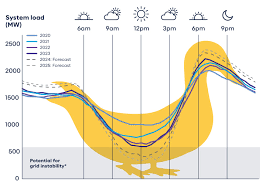
\includegraphics[width=1\linewidth]{duck.png}
        \caption{Duck curve- "La Duck Curve e la scomposizione della stagionalità dei
 consumi elettrici. Aspetti teorici e modelli statistici"-Bisetto Francesca}
        \label{fig:placeholder}
    \end{figure}
    \noindent
  \textbf{Renewable Energy Integration:} The most strategically significant contribution of V2G lies in addressing renewable energy intermittency challenges. V2G fleets function as large-scale energy buffers, absorbing excess solar and wind generation during periods of high production and low demand that would otherwise require curtailment. This stored renewable energy can subsequently be released during periods of low generation, such as evening hours or periods of limited wind availability. This mechanism directly increases the utilisation efficiency of renewable energy resources, supporting the integration objectives outlined in RED III while enhancing overall energy system efficiency \footcite{khan2024review, zou2021deep}.

\noindent
This vision is being actively incorporated into European legal frameworks and technical standards. The transformative \textbf{Alternative Fuels Infrastructure Regulation (AFIR, EU 2023/1804)} now requires that new public charging infrastructure incorporate smart charging capabilities and, critically, bidirectional power flow capacity. The technical implementation of these requirements is supported by standards such as \textbf{ISO 15118-20}, which provides detailed specifications for "Vehicle-to-Grid Communication Interface" (V2GCI) protocols, enabling secure, interoperable bidirectional power transfer. With mandatory implementation scheduled for 2027, the necessary technological and regulatory infrastructure is being systematically established. This regulatory push is supported by significant pilot initiatives including the \textbf{'SCALE'} and \textbf{'V2G Balearic Islands'} projects, which are conducting comprehensive testing of the technology's technical performance and economic viability under real-world operating conditions.

\noindent
Despite this regulatory progress, substantial obstacles to widespread V2G deployment persist. These challenges span technical, economic, and social dimensions:

\begin{itemize}
    \item \textbf{Market and Economic Barriers:} A coherent, pan-European framework for compensating EV owners for grid service provision remains undeveloped. While value streams exist within energy markets, accessing these markets involves significant complexity. Critical issues such as \textbf{"double taxation"} of electricity—where energy faces taxation both during charging and discharging phases—create substantial economic disincentives that require resolution through coordinated policy intervention.
    
    \item \textbf{Regulatory and Grid Access Challenges:} The recognition of EV fleets as qualified flexibility resources varies significantly across national electricity markets. Standardised procedures for grid interconnection, aggregator certification, secure data exchange protocols, and baseline calculation methodologies remain under development, creating a fragmented operational environment that complicates commercial deployment.
    
    \item \textbf{Technical and Consumer Adoption Barriers:} Consumer concerns regarding accelerated \textbf{battery degradation} and its implications for vehicle warranty coverage represent primary obstacles to participation. Additionally, the current installed base of EVs and charging infrastructure lacks universal bidirectional capability, although this limitation is being addressed through new vehicle platforms and evolving charging standards.
\end{itemize}
\noindent
The fundamental challenge addressed by this thesis extends beyond simply enabling V2G technology to encompass its \textit{intelligent orchestration}. This requires developing control strategies sophisticated enough to operate within emerging regulatory frameworks, navigate economic uncertainties, accommodate diverse user preferences, and overcome existing technical constraints. The objective is to unlock the substantial potential of EVs as fundamental components of Europe's energy transition while ensuring system reliability, economic viability, and user acceptance.
%%%%%%%%%%%%%%%%%%%%%%%%%%%%%%
%%%%%%%%%%%%%%%%%%%%%%%%%%%%%%

%%%%%%%%%%%%%%%%%%%%%%%%%%%%%%

%%%%%%%%%%%%%%%%%%%%%%%%%%%%%%


%%%%%%%%%%%%%%%%%%%%%%%%%%%%%%

%%%%%%%%%%%%%%%%%%%%%%%%%%%%%%
\section{The Optimizer's Trilemma: Navigating a Stochastic World}
\begin{center}
  \begin{minipage}{0.85\textwidth}
    \begin{displayquote}
      \large\itshape
      ``Uncertainty quantification provides a systematic way to assess the credibility of computational predictions.''
    \end{displayquote}
  \end{minipage}
\end{center}

\vspace{0.5cm}

\begin{flushright}
  --- \textsc{Omar Ghattas \& Karen Willcox}, \textit{Uncertainty Quantification in Computational Science and Engineering} (2016)
\end{flushright}
\noindent
While the potential of V2G technology is substantial, the management of distributed vehicular assets presents a complex control challenge. Economic viability drives aggregator decisions, yet a narrow focus on profitability alone proves insufficient for sustainable operations. Effective V2G management requires balancing three competing objectives that frequently conflict with one another. This challenge can be framed as the "V2G Optimizer's Trilemma": the concurrent pursuit of \textbf{economic profitability}, preservation of \textbf{battery longevity}, and maintenance of \textbf{user convenience}.
\noindent
Rather than representing a straightforward, static trade-off, this constitutes a dynamic, multi-objective optimisation challenge characterised by \textbf{stochasticity} and \textbf{uncertainty} arising from multiple, interconnected sources \footcite{wang2022multi}:
\\
    \noindent
    \textbf{Market Volatility:} Wholesale electricity prices exhibit significant variability driven by unpredictable supply variations (such as sudden reductions in wind generation capacity) and demand fluctuations (including heat-driven increases in cooling demand). Effective control systems must respond to these price signals dynamically and in real-time.
 \\
    \noindent   
\textbf{Renewable Intermittency:} Co-located solar and wind generation exhibit inherently variable output patterns with limited predictability. Controllers must coordinate EV fleet operations to capture available generation during surplus periods without compromising other operational objectives.
    \\
    \noindent
  \textbf{Human Behaviour:} Perhaps the most challenging uncertainty source involves EV owner patterns. Arrival times, departure schedules, and required state of charge (SoC) at departure lack deterministic characteristics. Emergency departures or unexpected schedule changes represent hard, non-negotiable constraints that intelligent systems must accommodate to preserve user trust and satisfaction.

\noindent
This dynamic, uncertain, and multifaceted operational environment renders static, rule-based control approaches (such as "charge when price falls below threshold X, discharge when exceeding threshold Y") inadequate and brittle. More sophisticated and adaptive methodologies are required—approaches capable of learning from operational experience and making optimal decisions under conditions of significant uncertainty. Reinforcement Learning excels in precisely this domain, providing a framework for developing control policies that demonstrate robustness, adaptability, and scalability.




%%%%%%%%%%%%%%%%%%%%%%%
\subsection{Sources for Energy Price Data}

Access to reliable, real-time, and historical market data remains crucial for both control agent training in simulation environments and real-world deployment. Key public sources for European market data include:
\\
\noindent
 \textbf{ENTSO-E Transparency Platform:} The European Network of Transmission System Operators for Electricity maintains a mandatory, open-access platform serving as a comprehensive repository of pan-European electricity market data. This includes harmonised day-ahead prices, load forecasts, and generation data, serving as the primary source for academic research through both web portal access and free RESTful API services.
    \\
\noindent
    \textbf{National Transmission System Operators (TSOs):} Many national TSOs (including Terna in Italy, National Grid in the UK, and RTE in France) publish detailed market data covering real-time frequency and imbalance prices for their respective jurisdictions.
    \\
\noindent
     \textbf{Power Exchanges:} Exchanges such as \textbf{EPEX SPOT} and \textbf{Nord Pool} constitute actual trading venues. While they represent direct price data sources, comprehensive real-time access typically requires commercial subscription services.


\subsection{Buying vs. Selling: The Critical Retail-Wholesale Spread}
\begin{center}
  \begin{minipage}{0.85\textwidth}
    \begin{displayquote}
      \large\itshape
      ``Price spreads, or marketing margins, are the difference between prices at different stages of the supply chain. 
      The wholesale-to-retail spread is the difference between the wholesale price and the retail price.''
    \end{displayquote}
  \end{minipage}
\end{center}

\vspace{0.5cm}

\begin{flushright}
  --- \textsc{Sebastien Pouliot \& Lee L. Schulz}, \textit{Measuring Price Spreads in Red Meat} (2016)
\end{flushright}
\noindent
A critical yet frequently overlooked aspect of V2G economics involves the distinction between EV owner charging costs and aggregator grid sales revenue.

\begin{itemize}
    \item \textbf{Selling Price (V2G Revenue):} When EVs provide energy to the grid, revenue calculation bases on \textbf{wholesale prices} (such as day-ahead spot prices). These prices reflect pure marginal energy costs at specific times.
    
    \item \textbf{Buying Price (Charging Cost):} End consumer EV charging costs reflect \textbf{retail prices}, significantly exceeding wholesale prices due to numerous non-energy components, termed "non-commodity costs":
    \begin{itemize}
        \item Base wholesale energy costs
        \item \textbf{Grid Tariffs:} Charges for high-voltage transmission and low-voltage distribution network usage
        \item \textbf{Taxes and Levies:} National or regional taxation including VAT and environmental levies applied to electricity consumption
        \item \textbf{Supplier Margin:} Retail energy provider profit margins
    \end{itemize}
\end{itemize}
\noindent
This substantial gap between retail purchasing prices and wholesale selling prices constitutes the "retail-wholesale spread," creating the primary opportunity for profitable energy arbitrage. For instance, with wholesale prices at €50/MWh and retail prices at €250/MWh, arbitrage operations achieve profitability only when selling prices exceed the full €250/MWh acquisition cost, not merely the €50/MWh wholesale component. Successful control strategies must account for these price differentials to enable economically rational decision-making.
\noindent
\\
A further perspective on this issue is provided by Parisio et al. 
\footcite{parisio2014mpc}
(2014), who develop a model predictive control (MPC) framework for microgrid operation. Their formulation explicitly considers the decision of when to buy from or sell to the utility grid, under time-varying spot prices and operational constraints. Importantly, the model prevents physically and economically unrealistic behaviors such as simultaneous buying and selling, and accounts for the real cost of storage and generation. This reinforces the notion that optimal energy management strategies must capture the full set of economic signals—including retail charges, network tariffs, and non-commodity costs—rather than relying solely on wholesale price arbitrage. In the V2G context, this highlights the need for predictive, multi-constraint optimization frameworks capable of managing battery limitations, retail–wholesale spreads, and market participation simultaneously in order to ensure profitability.
\newpage
\section{Modelling the V2G Ecosystem}
\label{sec:ev_and_scenario}

Before examining control algorithms, establishing clear, high-fidelity models of system core components becomes essential: the electric vehicle as a controllable cyber-physical asset, and the operational environment or "scenario." The interaction between these elements defines V2G optimisation task boundaries and objectives.

\subsection{The Grid-Interactive EV as a Controllable Asset}

\begin{center}
  \begin{minipage}{0.85\textwidth}
    \begin{displayquote}
      \large\itshape
      "Electric car sales continue to break records globally, particularly in China and other emerging economies."\\[1em]

    \end{displayquote} 
    
  \end{minipage} 
\end{center}

\begin{flushright}
  \textsc{\textbf{International Energy Agency (IEA)}
\footnote{\href{https://www.iea.org/reports/global-ev-outlook-2025/executive-summary}{Global EV Outlook 2025 - Executive Summary}}}
\end{flushright}



\noindent
From a power grid perspective, electric vehicles represent sophisticated mobile energy storage devices. For V2G applications, EVs can be characterised through several key state variables and parameters:
\\
\noindent
    \textbf{The Battery:} The core grid asset component, defined by \textbf{nominal energy capacity} (in kWh), current \textbf{State of Charge (SoC)}, and \textbf{State of Health (SoH)} representing degradation over time. Operation is constrained by \textbf{power limits} (in kW) dictating maximum charge or discharge rates, and charging/discharging \textbf{efficiencies} accounting for energy losses.
    \\
    \noindent
    \textbf{The On-Board Charger (OBC):} For AC charging applications, the OBC converts grid alternating current to battery direct current. Power rating often constitutes the primary bottleneck for both charging and V2G power output.
    \\
\noindent    
  \textbf{Communication Interface:} V2G participation requires vehicle-charging station (EVSE) communication capabilities. This is governed by standards including \textbf{ISO 15118} and protocols such as the \textbf{Open Charge Point Protocol (OCPP)}, enabling secure information exchange required for smart and bidirectional power flow operations.
\\
\noindent
Combined with vehicle availability patterns—arrival and departure times plus user energy requirements—these characteristics transform EVs from simple loads into fully dispatchable grid resources.
\newpage
%%%%%%%%%%%%%%%%%%%%%%%%%%%%%%%%%%%%%
%%%%%%%%%%%%%%%%%%%%%%%%%%%%%%%%%%%%%%%%
%%%%%%%%%%%%%%%%%%%%%%%%\section{A New Paradigm for Control: Reinforcement Learning}

\section{A New Paradigm for Control: Reinforcement Learning - Based on the work of Sutton \& Barto}



\begin{center}
    \begin{minipage}{0.85\textwidth}
        \large\itshape
        ``Reinforcement learning is learning what to do---how to map situations to actions---so as to maximize a numerical reward signal.''
    \end{minipage}
\end{center}

\vspace{0.5cm}

\begin{flushright}
--- Richard S. Sutton \& Andrew G. Barto, \textit{Reinforcement Learning: An Introduction} (2018) \cite{Sutton2018}
\end{flushright}

\noindent
To address the complexities of uncertainty, multi-objective trade-offs, and dynamic systems, this work employs Reinforcement Learning (RL), a machine learning paradigm that learns optimal sequential decision-making policies through trial-and-error interaction with an environment. Unlike traditional optimal control methods, which depend on an explicit and accurate model of the environment's dynamics, RL agents learn directly from the outcomes of their actions. This model-free approach provides significant robustness in the face of uncertainty and unmodeled dynamics.

\section{The Reinforcement Learning Problem}
The problem of reinforcement learning is formalized as the interaction between a learning \textbf{agent} and its \textbf{environment}. This interaction unfolds over a sequence of discrete time steps, $t = 0, 1, 2, \dots$.

\subsection{The Agent-Environment Interface}
At each time step $t$, the agent receives a representation of the environment's \textbf{state}, $S_t \in \mathcal{S}$, and on that basis selects an \textbf{action}, $A_t \in \mathcal{A}(S_t)$. One time step later, as a consequence of its action, the agent receives a numerical \textbf{reward}, $R_{t+1} \in \mathcal{R}$, and finds itself in a new state, $S_{t+1}$. This interaction loop forms the foundational framework of the RL problem.

\begin{figure}[h!]
    \centering
    % Placeholder for a standard RL interaction diagram
    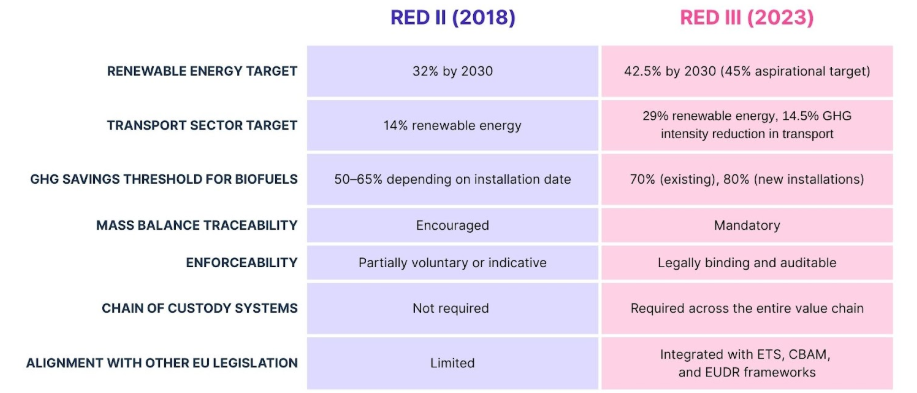
\includegraphics[width=0.8\linewidth]{red.png}
    \caption{The agent-environment interaction loop in reinforcement learning \cite{Sutton2018}.}
    \label{fig:rl_loop}
\end{figure}

\subsection{Goals, Rewards, and Returns}
The agent's objective is formalized by the \textbf{reward hypothesis}: that all goals and purposes can be framed as the maximization of the expected cumulative reward. The agent's goal is not to maximize the immediate reward, $R_{t+1}$, but the cumulative reward in the long run. This cumulative reward is known as the \textbf{return}, denoted $G_t$.

For \textit{episodic tasks} that terminate, the return is the finite sum of future rewards. For \textit{continuing tasks} that do not terminate, the return is defined as the discounted sum of future rewards:
\begin{equation}
    G_t \doteq \sum_{k=0}^{\infty} \gamma^k R_{t+k+1}
\end{equation}
where $\gamma \in [0, 1)$ is the \textbf{discount factor}. It determines the present value of future rewards, ensuring the infinite sum is finite and balancing immediate gratification against long-term gains. A value of $\gamma=0$ results in a myopic agent concerned only with maximizing immediate rewards.

\section{The Language of Learning: Markov Decision Processes}
The mathematical foundation of RL is the \textbf{Markov Decision Process (MDP)}, a formal framework for modeling decision-making in stochastic environments where outcomes are partly random and partly under the control of a decision maker.

\subsection{The Markov Property}
The future is independent of the past given the present. A state signal $S_t$ is said to have the \textbf{Markov Property} if the environment's response at time $t+1$ depends only on the state and action at time $t$. The probability of transitioning to state $s'$ and receiving reward $r$ is independent of all previous states and actions:
\begin{equation}
    p(s', r | s, a) \doteq \Pr\{S_{t+1}=s', R_{t+1}=r | S_t=s, A_t=a\}
\end{equation}
This property is fundamental as it allows decisions to be made based solely on the current state, without needing the complete history of interaction.

\subsection{Policies and Value Functions}
The agent's learning objective is to find a good \textbf{policy}, $\pi(a|s)$, which is a mapping from states to probabilities of selecting each possible action. The goodness of a policy is assessed by its \textbf{value functions}.
\begin{itemize}
    \item The \textbf{state-value function}, $v_\pi(s)$, is the expected return starting from state $s$ and following policy $\pi$ thereafter:
    \begin{equation}
        v_\pi(s) \doteq \mathbb{E}_\pi [G_t | S_t=s]
    \end{equation}
    \item The \textbf{action-value function}, $q_\pi(s, a)$, is the expected return starting from state $s$, taking action $a$, and thereafter following policy $\pi$:
    \begin{equation}
        q_\pi(s, a) \doteq \mathbb{E}_\pi [G_t | S_t=s, A_t=a]
    \end{equation}
\end{itemize}

\section{The Bellman Equations}
The Bellman equations provide a recursive decomposition that is foundational to solving MDPs. They express the value of a state in terms of the values of its successor states.

\subsection{The Bellman Expectation Equation}
For a given policy $\pi$, the state-value function must satisfy a self-consistency condition. The value of a state equals the expected immediate reward plus the discounted expected value of the next state:
\begin{equation}
    v_\pi(s) = \sum_a \pi(a|s) \sum_{s', r} p(s', r | s, a) [r + \gamma v_\pi(s')]
\end{equation}
This is the \textbf{Bellman expectation equation} for $v_\pi$. It forms the basis for policy evaluation algorithms.

\subsection{The Bellman Optimality Equation}
The ultimate goal is to find an \textbf{optimal policy}, $\pi_*$, which is a policy that achieves a higher or equal expected return than all other policies from all states. All optimal policies share the same optimal value functions, $v_*(s)$ and $q_*(s, a)$. The optimal value function for a state is the maximum expected return achievable from that state:
\begin{equation}
    v_*(s) = \max_a \mathbb{E}[R_{t+1} + \gamma v_*(S_{t+1}) | S_t=s, A_t=a] = \max_a \sum_{s', r} p(s', r | s, a) [r + \gamma v_*(s')]
\end{equation}
This is the \textbf{Bellman optimality equation}. Solving it means finding the optimal policy.

\section{Solution Methods: A Unified Perspective}
\subsection{Generalized Policy Iteration (GPI)}
Most RL algorithms can be understood within the framework of \textbf{Generalized Policy Iteration (GPI)}, as described in Chapter 4 of \cite{Sutton2018}. GPI refers to the general idea of letting two interacting processes, policy evaluation and policy improvement, work towards a common optimal solution.

\begin{itemize}
    \item \textbf{Policy Evaluation}: Given a policy $\pi$, compute its value function $v_\pi$. This step aims to make the value function consistent with the current policy.
    \item \textbf{Policy Improvement}: Given a value function $v$, improve the policy by making it greedy with respect to $v$. For a given state $s$, the new policy will select the action $a$ that maximizes $q_\pi(s, a)$.
\end{itemize}

These two processes compete in the short term (improving the policy makes the value function inaccurate) but cooperate in the long term to converge to the optimal policy and optimal value function. \textbf{Dynamic Programming (DP)} methods like policy iteration and value iteration are classic examples of GPI, assuming a perfect model of the environment.

\section{Learning from Experience: MC and TD Methods}
When a model of the environment is not available, we must learn from sampled experience. Chapters 5 and 6 of \cite{Sutton2018} introduce two primary model-free approaches.

\subsection{Monte Carlo (MC) Methods}
MC methods learn value functions by averaging the returns from sample episodes.
\begin{itemize}
    \item \textbf{Principle}: An update to $V(S_t)$ is made only at the end of an episode.
    \item \textbf{Update Target}: The target for the update is the actual, complete return $G_t$.
    \item \textbf{Update Rule} (Constant-$\alpha$): $V(S_t) \leftarrow V(S_t) + \alpha [G_t - V(S_t)]$
    \item \textbf{Properties}: MC methods are unbiased but can have high variance and are only applicable to episodic tasks. They do not \textit{bootstrap}.
\end{itemize}

\subsection{Temporal-Difference (TD) Learning}
TD learning is a central and novel idea in RL, combining ideas from both MC and DP.
\begin{itemize}
    \item \textbf{Principle}: TD methods update the value estimate for a state based on the observed reward and the estimated value of the successor state. They learn from incomplete episodes.
    \item \textbf{Update Target}: The target is an estimate of the return, called the TD Target: $R_{t+1} + \gamma V(S_{t+1})$.
    \item \textbf{Update Rule} (TD(0)): $V(S_t) \leftarrow V(S_t) + \alpha [R_{t+1} + \gamma V(S_{t+1}) - V(S_t)]$
    \item \textbf{Properties}: TD methods \textit{bootstrap}—they update a guess from a guess. This introduces bias but often leads to lower variance and faster learning. They are naturally implemented in an online, fully incremental fashion.
\end{itemize}

\section{Actor-Critic Architectures}
The \textbf{Actor-Critic} architecture provides a powerful and widely adopted method for solving RL problems, particularly in continuous action spaces. It explicitly represents both the policy and the value function using two distinct function approximators (e.g., neural networks).

\begin{itemize}
    \item \textbf{The Critic}: Learns a value function (e.g., $v_\pi(s)$ or $q_\pi(s, a)$). Its role is to evaluate the actor's decisions by computing the TD error:
    \begin{equation}
        \delta_t = R_{t+1} + \gamma V(S_{t+1}) - V(S_t)
    \end{equation}
    \item \textbf{The Actor}: Represents the policy, $\pi_\theta(a|s)$, parameterized by $\theta$. It receives the current state as input and outputs an action. It uses the TD error from the critic as a learning signal to update its parameters via policy gradient methods, improving its strategy over time.
\end{itemize}

This separation of concerns allows for direct policy optimization in continuous or large action spaces while leveraging the stable learning dynamics of TD-based value estimation.
% ===================================================================
% REWARD SHAPING SECTION
% ===================================================================
 \section{Reward Engineering: Shaping Agent Behavior}
\label{sec:reward_shaping}

The reward function is arguably the most critical component in a Reinforcement Learning system. It is the sole mechanism through which a designer can communicate the desired behavior to the agent. A poorly designed reward can lead to unintended and suboptimal behaviors, even if the agent successfully maximizes it. The entire field of reward engineering has become a cornerstone of modern RL, as it is fundamental to applying these algorithms effectively in complex, real-world applications \footcite{ibrahim2024comprehensive}. The V2G problem, with its multiple competing objectives—maximizing profit, ensuring user satisfaction, preserving battery health, and maintaining grid stability—makes reward design particularly challenging. This work explores several sophisticated techniques to guide the learning process effectively.

\subsection{Potential-Based Reward Shaping (PBRS)}
Potential-Based Reward Shaping (PBRS) is perhaps the most theoretically sound method for reward augmentation \footcite{ng1999policy}. It involves adding a shaping term, $F(s, s')$, to the environment's intrinsic reward, $R(s, a, s')$. The new, shaped reward $R'$ is thus defined as:
\[
R'(s, a, s') = R(s, a, s') + F(s, s')
\]
The shaping term itself is defined as the difference between a potential function, $\Phi$, evaluated at the new state and the old state:
\[
F(s, s') = \gamma \Phi(s') - \Phi(s)
\]
where $\gamma$ is the discount factor. The key theoretical guarantee of PBRS is \textbf{policy invariance}: adding a potential-based shaping reward does not change the optimal policy of the underlying MDP. While the agent learns the same optimal behavior, the shaping term can provide dense, intermediate rewards that significantly accelerate the learning process by guiding the agent's exploration.

\subsection{Dynamic and Adaptive Rewards}
Unlike PBRS, which provides a static reward bonus, a dynamic or adaptive reward function can evolve during training. This approach is particularly useful for complex problems where the relative importance of different objectives may change as the agent becomes more competent. For example, an agent could initially be rewarded simply for keeping an EV charged, but as training progresses, the reward function could adapt to introduce penalties for grid overloads or incentives for V2G services \footcite{wan2022dynamic}. This allows the agent to master different facets of the problem sequentially.

\subsection{Curriculum Learning}
While technically a training paradigm rather than a reward modification technique, Curriculum Learning (CL) is highly relevant to reward engineering. CL involves training the agent on a sequence of tasks that gradually increase in difficulty. In the V2G context, an agent might first be trained in a simple scenario with only a few EVs and stable prices. Once it masters this, it is moved to a more complex environment with more EVs, volatile prices, and hard constraints. This structured learning process prevents the agent from being overwhelmed by the full complexity of the problem from the start and can lead to more robust and generalizable policies.

\newpage
\section{The Rise of Deep Reinforcement Learning for V2G Control}

The convergence of RL with the substantial representational capabilities of deep neural networks has given rise to \textbf{Deep Reinforcement Learning (DRL)}, which currently represents the leading edge of V2G control research. The development of DRL algorithms has yielded a comprehensive toolkit, primarily divided into two main families: off-policy and on-policy methods, each exhibiting distinct operational characteristics.
The following figure illustrates the evolutionary relationships between the algorithms that  will be discussed, highlighting how newer ideas were built to overcome the limitations of their predecessors.

\begin{forest}
for tree={
grow=east,
parent anchor=east,
child anchor=west,
edge path={
\noexpand\path [draw] (!u.parent anchor) -- +(-0.5pt,0) |- (.child anchor)\forestoption{edge label};
},
draw,
rounded corners,
align=center,
l sep=7pt,
s sep=4pt,
minimum height=0.4cm,
inner sep=0.1pt,
anchor=west,
}
[RL Methods
[On-Policy
[Policy Gradient
[A2C]
[TRPO\\(Theoretical Stability)
[PPO\\(Practical Simplification)]
]
]
[Gradient-Free
[ARS\\(Random Search)]
]
]
[Off-Policy\\
[DDPG\\(Fundamental)
[DDPG+PER\\(Improve Sampling)]
[TD3\\(Resolve Overestimation)]
[SAC\\(Add Entropy)]
[TQC\\(Distributional Approach)]
]
]
]
\end{forest}
\subsection{Off-Policy Methods: Data-Efficient Learning from Experience}

Off-policy algorithms distinguish themselves through their capacity to learn optimal policies from data generated by different, often more exploratory, behavioral policies. This enables them to reuse historical experiences stored in large \textit{replay buffers}, breaking temporal correlation between experiences and achieving high sample efficiency.

\paragraph{Deep Deterministic Policy Gradient (DDPG)}

A foundational algorithm that successfully extended Deep Q-Networks (DQN) to high-dimensional, continuous action spaces, DDPG represented a significant breakthrough for control problems including V2G \footcite{lillicrap2015continuous}. It employs an actor-critic architecture where the actor deterministically maps states to actions. However, practical applications often encounter substantial training instability and systematic vulnerability to \textbf{overestimation bias}, where critic networks systematically overestimate Q-values, resulting in suboptimal policy learning \footcite{orfanoudakis2022deep, alfaverh2022optima}.

\paragraph{Twin Delayed DDPG (TD3)}

Developed as a direct successor to address DDPG's instabilities, TD3 introduces three key innovations that have become standard in contemporary DRL \footcite{fujimoto2018addressing}. It incorporates (1) clipped double Q-learning, utilizing paired critic networks and selecting minimum estimates to mitigate overestimation bias; (2) delayed policy updates, updating actors less frequently than critics for enhanced stability; and (3) target policy smoothing, adding noise to target actions for learning regularization. These enhancements establish TD3 as a more robust and reliable baseline for complex V2G applications \footcite{liu2023optimal, wang2022multi}.

\paragraph{Soft Actor-Critic (SAC)}

SAC represents a state-of-the-art off-policy algorithm for continuous control, recognized for superior sample efficiency and stability \footcite{haarnoja2019soft}. Its fundamental innovation involves the \textbf{maximum entropy framework}. The agent's objective is modified to maximize both expected reward and policy entropy. This entropy bonus encourages agents to act as randomly as possible while maintaining task success, promoting broader exploration, improved noise robustness, and reduced risk of poor local optima convergence \footcite{logeshwaran2022comparative}.

\paragraph{Truncated Quantile Critics (TQC)}

TQC addresses overestimation bias through a distributional RL approach \footcite{kuznetsov2020controlling}. Rather than learning single expected returns (Q-values), its critic learns complete return probability distributions using quantile regression. By learning multiple return distribution quantiles and truncating the most optimistic quantile estimates before averaging, it provides a more principled and effective method for removing primary overestimation bias sources, frequently achieving superior performance.

\paragraph{Enhancement: Prioritized Experience Replay (PER)}

This represents not a standalone algorithm but a crucial orthogonal modification for off-policy methods. Standard replay buffers sample past transitions uniformly. PER samples transitions based on their "importance," typically proportional to TD error magnitude \footcite{schaul2015prioritized}. This focuses learning processes on surprising or informative experiences, significantly accelerating convergence and improving final performance.

\subsection{On-Policy Methods: Stability through Cautious Updates}

On-policy methods learn exclusively from data generated by current policies being optimized. Once data is used for updates, it is discarded. While this makes them inherently less sample-efficient than off-policy counterparts, their updates often demonstrate greater stability and reduced divergence risk.

\paragraph{Advantage Actor-Critic (A2C/A3C)}

A2C represents a foundational synchronous, on-policy Actor-Critic algorithm. Its powerful extension, \textbf{Asynchronous Advantage Actor-Critic (A3C)}, was a landmark contribution demonstrating parallelism benefits \footcite{mnih2016asynchronous}. A3C utilizes multiple parallel workers, each with individual model and environment copies. These workers interact with their environments independently, and collected gradients update a global model asynchronously. This decorrelates data streams and provides powerful stabilizing effects on learning processes.

\paragraph{Trust Region Policy Optimization (TRPO)}

TRPO was the first algorithm to formalize policy update size constraints for guaranteed monotonic policy improvement \footcite{schulman2020trust}. It maximizes a "surrogate" objective function subject to policy change constraints, measured by Kullback-Leibler (KL) divergence. This creates a "trust region" within which new policies are guaranteed to improve upon previous ones, preventing catastrophic updates that can permanently derail learning. However, implementation complexity arises from second-order optimization requirements.

\paragraph{Proximal Policy Optimization (PPO)}

PPO achieves TRPO's stability benefits and reliable performance using only first-order optimization, making it far simpler to implement and more broadly applicable \footcite{schulman2017proximal}. It employs a novel \textbf{clipping} mechanism in its objective function to discourage large policy updates that would move new policies too far from previous ones, effectively creating "soft" trust regions. Due to its excellent balance of performance, stability, and implementation simplicity, PPO has become a default choice for many on-policy applications.

\subsection{Gradient-Free Methods: An Alternative Path}

\paragraph{Augmented Random Search (ARS)}

As a counterpoint to dominant gradient-based methods, ARS represents a gradient-free approach that optimizes policies directly in parameter space \footcite{mania2018simple}. It operates by exploring random policy parameter perturbations and updating central policy parameter vectors based on observed performance of these perturbations. While often less sample-efficient for complex, high-dimensional problems, its extreme simplicity, scalability, and robustness to noisy rewards can make it competitive in certain domains.

\section{The Model-Based Benchmark: Model Predictive Control (MPC)}

While DRL offers powerful model-free approaches, model based techniques  requires benchmarking against its most robust model-based counterpart: \textbf{Model Predictive Control (MPC)}. MPC originated in the 1970s within the process control industry, with pioneering contributions by Richalet et al. \footcite{Richalet1978ModelPH} and Cutler and Ramaker \footcite{Cutler1980}. The theoretical foundations for stability and optimality were subsequently established rigorously by researchers including Mayne and Rawlings \footcite{mayne2000constraine}.
\noindent
At its core, MPC represents a proactive, forward-looking strategy that employs explicit mathematical system models to predict future evolution. At each control step, it solves finite-horizon optimal control problems to determine optimal control action sequences. Its primary strength, explaining widespread industrial adoption, lies in its inherent capability to proactively handle complex system dynamics and operational constraints \footcite{minchala2025systematic}.
\section{Model Predictive Control Formulation}
\textit{Section based on "Predictive Control for Linear and Hybrid Systems" by F. Borrelli, A. Bemporad, and M. Morari.}

\subsection{The Finite Time Optimal Control Problem}

At each time step $t$, given the current state measurement $x(t)$, a Model Predictive Control (MPC) law is defined by solving a constrained finite time optimal control problem. This is often referred to as Receding Horizon Control (RHC).
\noindent
Consider the discrete-time linear time-invariant system:
\begin{equation}
    x(k+1) = Ax(k) + Bu(k)
\end{equation}
The optimization problem solved at the current time $t$ is formulated as follows, using $x(t)$ as the initial state $x_0$:

\begin{equation}
    J_0^*(x(t)) = \min_{U_0} J_0(x(t), U_0)
\end{equation}
where the cost function $J_0$ for a quadratic objective is defined as:
\begin{equation}
    J_0(x(0), U_0) = x_N' P x_N + \sum_{k=0}^{N-1} (x_k'Qx_k + u_k'Ru_k)
\end{equation}
The minimization is subject to the following constraints for $k=0, \dots, N-1$:
\begin{align}
    \text{subj. to} \quad x_{k+1} &= Ax_k + Bu_k, \\
    x_k &\in \mathcal{X}, \\
    u_k &\in \mathcal{U}, \\
    x_N &\in \mathcal{X}_f, \\
    x_0 &= x(t).
\end{align}
Here, the variables are defined as:
\begin{itemize}
    \item $x_k \in \mathbb{R}^n$ denotes the state vector at time $k$ obtained by starting from the state $x_0 = x(t)$ and applying the input sequence $u_0, \dots, u_{k-1}$.
    \item $U_0 = [u_0', \dots, u_{N-1}']' \in \mathbb{R}^{mN}$ is the decision vector containing all future inputs over the prediction horizon $N$.
    \item $P, Q$ are positive semi-definite state penalty matrices, and $R$ is a positive definite input penalty matrix.
    \item $\mathcal{X} \subseteq \mathbb{R}^n$ and $\mathcal{U} \subseteq \mathbb{R}^m$ are polyhedra representing state and input constraints, respectively.
    \item $\mathcal{X}_f \subseteq \mathbb{R}^n$ is a terminal polyhedral region that the state $x_N$ is constrained to enter.
\end{itemize}

\subsection{The Receding Horizon Policy}

The optimization problem yields an optimal sequence of control inputs $U_0^*(x(t)) = \{u_0^*, u_1^*, \dots, u_{N-1}^*\}$.
In the receding horizon control strategy, only the first element of this sequence is applied to the system:
\begin{equation}
    u(t) = u_0^*(x(t))
\end{equation}
At the next time step, $t+1$, a new state measurement $x(t+1)$ is obtained. The entire optimization problem is then solved again over a shifted horizon $[t+1, t+1+N]$, using $x(t+1)$ as the new initial state. This process is repeated at each sampling instant.


%%%%%%%%%%%%
\subsection{Implicit MPC: Online Optimization}

The most common formulation involves \textbf{Implicit MPC}, where constrained optimization problems are solved online at each control step. For linear systems with quadratic costs, this typically constitutes a Quadratic Program (QP). The controller's objective involves finding future control input sequences 
\[
U = [u_{t|t}, \dots, u_{t+N-1|t}]
\] 
that minimize a cost function $J$ over a prediction horizon $N$.
\noindent
A key insight from \cite{borrelli2017predictive} is that in this formulation, the control law is defined \textbf{implicitly} as the result of an optimization problem. There is no pre-computed algebraic function; the control action is discovered at each step through a numerical computation. This approach is powerful due to its directness but is fundamentally limited by the need to perform this computation online. The authors of \cite{borrelli2017predictive} highlight this on page xii, stating: 
\begin{quote}
“One limitation of MPC is that running the optimization algorithm on-line at each time step requires substantial time and computational resources.”
\end{quote}
\noindent
The finite-horizon optimal control problem is formulated as:
\begin{equation}
\min_{U_t} J(x_t, U_t) = \sum_{k=0}^{N-1} \left( x_{t+k|t}^\top \mathbf{Q} x_{t+k|t} + u_{t+k|t}^\top \mathbf{R} u_{t+k|t} \right) + x_{t+N|t}^\top \mathbf{P} x_{t+N|t}
\end{equation}
where $x_{t+k|t}$ represents the predicted state at future step $k$ based on information at time $t$, and $\mathbf{Q}$, $\mathbf{R}$, and $\mathbf{P}$ are weighting matrices defining trade-offs between state deviation and control effort. This optimization is subject to system dynamics and operational constraints:
\begin{align}
x_{t+k+1|t} &= \mathbf{A} x_{t+k|t} + \mathbf{B} u_{t+k|t} \\
x_{\min} \leq\ &x_{t+k|t} \leq x_{\max} \\
u_{\min} \leq\ &u_{t+k|t} \leq u_{\max}
\end{align}
\noindent
At each time step $t$, this complete problem is solved, but only the first action of the optimal sequence, $u_{t|t}^*$, is applied to the system. The process then repeats at the next time step, $t+1$, using new system state measurements. This feedback mechanism, known as a \textit{receding horizon} strategy, makes MPC robust to disturbances and model mismatch \cite{camacho2013model}.


\section{Improvement of the Standard Fixed-Horizon MPC Formulation}

Model Predictive Control (MPC) addresses the control of a discrete-time nonlinear system, as described in \cite{krener2016adaptive}:
\begin{equation}
    x^{+} = f(x, u)
    \label{eq:system}
\end{equation}
where $x \in \mathbb{R}^n$ is the state and $u \in \mathbb{R}^m$ is the control input. The objective is to solve a finite-horizon optimal control problem at each time step. For a \textbf{fixed prediction horizon} $N$, the problem is formulated as finding a control sequence $u_N = (u(0), \dots, u(N-1))$ that minimizes a cost function, defined in eq. (11) of the paper as:
\begin{equation}
    V_N(x) = \sum_{k=0}^{N-1} l(x(k), u(k)) + V_f(x(N))
    \label{eq:cost}
\end{equation}
This minimization is subject to system dynamics, state and input constraints, and the crucial terminal constraint $x(N) \in \mathcal{X}_f$. Here, $\mathcal{X}_f$ is a terminal set where stability is guaranteed, and $V_f(x)$ is a terminal cost that acts as a control Lyapunov function on $\mathcal{X}_f$ \cite{krener2016adaptive}.

\subsection{Limitation of the Fixed-Horizon Approach}
The primary drawback of this standard formulation is the static nature of the horizon $N$. The choice of $N$ represents a difficult compromise. As Krener points out on page 2, "One would expect when the current state $x$ is far from the operating point, a relatively long horizon $N$ is needed... but as the state approaches the operating point shorter and shorter horizons can be used" \cite{krener2016adaptive}. A fixed horizon long enough for the worst-case scenario is computationally wasteful for the majority of the operational time, as it increases the dimensionality of the optimization problem ($m \times N$) solved online.

\section{Improving the Formulation with Adaptive Horizon MPC (AHMPC)}

The core innovation of Adaptive Horizon Model Predictive Control (AHMPC) is to make the horizon length state-dependent, adapting it online to be as short as possible while maintaining stability.

\subsection{The Ideal (but Impractical) AHMPC Scheme}
The paper first introduces an "ideal" version of AHMPC. This scheme relies on a function $N(x)$, defined as the minimum integer $N$ for which a feasible control sequence exists that drives the state $x$ into the terminal set $\mathcal{X}_f$ (see Assumption 4 in \cite{krener2016adaptive}). The resulting optimal cost and control law are then state-dependent through this horizon:
\begin{align}
    V(x) &= V_{N(x)}(x) \label{eq:ideal_cost} \\
    \kappa(x) &= \kappa_{N(x)}(x) \label{eq:ideal_control}
\end{align}
As shown in Section II of the paper, this formulation leads to a valid Lyapunov function, confirming its stabilizing properties. However, this scheme is impractical because "in general, it is impossible to compute the function $N(x)$" \cite{krener2016adaptive}.

\subsection{The Practical AHMPC Algorithm}
Section III of the paper presents a practical algorithm that circumvents the need to know $N(x)$ or even the terminal set $\mathcal{X}_f$ explicitly. The key idea is to use the terminal controller $\kappa_f(x)$ and terminal cost $V_f(x)$ to \textit{verify online} if the chosen horizon is sufficient.
\\
\noindent
At a given state $x$ and with a current horizon guess $N$, the algorithm is as follows:
\begin{enumerate}
    \item \textbf{Solve and Extend:} Solve the N-horizon optimal control problem to get the trajectory $x^0(\cdot)$. Then, extend this trajectory for $L$ additional steps using the terminal feedback law:
    \begin{equation}
        x^0(k+1) = f(x^0(k), \kappa_f(x^0(k))), \quad \text{for } k = N, \dots, N+L-1
    \end{equation}
    
    \item \textbf{Verify Stability Conditions:} Check if the Lyapunov conditions, given as equations (18) and (19) in \cite{krener2016adaptive}, hold along this extended part of the trajectory:
    \begin{align}
        V_f(x^0(k)) &\ge \alpha(|x^0(k)|) \\
        V_f(x^0(k)) - V_f(x^0(k+1)) &\ge \alpha(|x^0(k)|)
    \end{align}
    for $k = N, \dots, N+L-1$. Failure to satisfy these conditions implies that the terminal state $x^0(N)$ is likely not in a region of stability.
    
    \item \textbf{Adapt the Horizon:} The adaptation logic is described on page 5 of the paper:
    \begin{itemize}
        \item \textbf{If conditions hold:} The horizon $N$ is considered sufficient. The control $u^0(0)$ is applied. At the next state $x^+$, the controller attempts a shorter horizon, typically $N-1$.
        \item \textbf{If conditions fail:} The horizon $N$ is too short. The controller "increase[s] N by 1 and... solve[s] the optimal control problem over the new horizon" from the same state $x$ \cite{krener2016adaptive}. This is repeated until a sufficient horizon is found.
    \end{itemize}
\end{enumerate}

\subsection{Advantages of the AHMPC Formulation}
This practical scheme offers significant advantages, as highlighted in the paper's conclusion:
\begin{itemize}
    \item \textbf{Computational Efficiency:} The primary advantage is that "the AHMPC horizon length decreases as the process is stabilized thereby lessening the on-line computational burden" \cite{krener2016adaptive}.
    \item \textbf{No Explicit Terminal Set:} The algorithm cleverly "proceeds without knowing the minimum horizon length function $N(x)$ and without knowing the domain of Lyapunov stability of the terminal cost $V_f(x)$" \cite{krener2016adaptive}. This removes a major hurdle in traditional MPC design.
\end{itemize}

\section{Further Enhancements via Learning-Based Approaches}

While the practical AHMPC algorithm provides a significant advantage, it still relies on an iterative, trial-and-error process of increasing $N$ when the current horizon is insufficient. This can introduce computational delays.
\\
\noindent
Modern data-driven techniques, such as Deep Reinforcement Learning (DRL), offer a path to mitigate this. DRL has proven effective for learning complex control policies for challenging problems, such as managing Electric Vehicle charging in volatile markets \cite{orfanoudakis2022deep}. A hybrid approach could be envisioned where a DRL agent is trained offline to approximate the ideal horizon function $N(x)$. This learned function would provide a highly accurate initial guess for the horizon at each step, potentially eliminating the need for online iterative adjustments and combining the computational speed of a learned policy with the rigorous stability and constraint-handling framework of AHMPC.




%%%%%%%%%%%%%%%%%%%
%%%%%%%%%%%%%%%%%%%%%%
\section{Explicit MPC: Offline Pre-computation}

For systems with fast dynamics or limited online computational capacity, \textbf{Explicit MPC} offers an alternative approach. The key idea is to move the computational effort entirely offline. As detailed extensively in \cite{borrelli2017predictive}, this is achieved by treating the current state $x_t$ not as a fixed value, but as a vector of parameters. The constrained optimization problem is then solved offline for all possible initial states within a given range using \textbf{multi-parametric programming}.

\noindent
The authors of \cite{borrelli2017predictive} frame this as the main contribution of their work (Preface, page xii): 
\begin{quote}
“we want to determine the [...] feedback control law $f(x)$ that generates the optimal $u_k = f(x(k))$ \textbf{explicitly} and not just \textbf{implicitly} as the result of an optimization problem.”
\end{quote}
\noindent
The result is not an online algorithm, but a pre-computed, explicit control law, $K(x_t)$, which for linear systems is a \textbf{piecewise affine (PWA) function} of the state vector $x_t$:
\begin{equation}
u^*(x_t) = \mathbf{F}_i x_t + \mathbf{g}_i \quad \text{if } x_t \in \mathcal{X}_i
\end{equation}
\noindent
The state space is partitioned into a set of convex polyhedral regions $\mathcal{X}_i$, with a unique affine control law defined for each region. Online operation is thereby reduced from solving a QP to a simple function evaluation: first, a fast lookup operation identifies which region $\mathcal{X}_i$ the current state $x_t$ occupies, and second, the corresponding simple affine control law is applied. This trades a very high offline computational burden and significant memory requirements for extremely fast and deterministic online execution \cite{bemporad2013explicit, borrelli2017predictive}.
\subsection{Deep Learning for an Efficient Explicit MPC Representation}

While implicit MPC provides an optimal control action, its reliance on solving a numerical optimization problem at each sampling time makes it unsuitable for systems with fast dynamics. An alternative is Explicit MPC, where the control law---a Piecewise Affine (PWA) function of the state---is pre-computed offline. However, this approach suffers from a significant drawback: the number of polyhedral regions, and thus the memory required to store the corresponding affine laws, can grow exponentially with the prediction horizon and the number of constraints \cite{karg2018efficient}. This "curse of dimensionality" severely limits its practical application, especially in memory-constrained embedded systems.

To address this challenge, the work in \cite{karg2018efficient} proposes a novel approach that leverages deep learning to create a highly efficient representation of the explicit MPC law. The methodology bridges the gap between the implicit and explicit approaches by using the former to train the latter.

\subsubsection{Training via Implicit MPC Data Generation}
The core idea is to train a deep neural network to act as the explicit controller. This requires a comprehensive dataset of optimal state-action pairs, which is generated in a crucial offline phase. As detailed in \cite{karg2018efficient}, this is achieved by repeatedly using the \textbf{implicit MPC solver}:
\begin{enumerate}
    \item A large number of state points ($x_{tr,i}$) are sampled from the relevant operating region of the system.
    \item For each state point, the full MPC optimization problem (a Quadratic Program, or QP) is solved to find the corresponding optimal control input ($u^*_{tr,i}$). This is precisely the task an implicit MPC controller performs online.
    \item The resulting pairs $(x_{tr,i}, u^*_{tr,i})$ form a large dataset that effectively maps states to their optimal control actions.
\end{enumerate}
This dataset is then used to train a deep neural network via supervised learning, minimizing the error between the network's output and the optimal control actions. In essence, the computationally intensive implicit solver is used offline to "teach" a fast and compact neural network how to behave optimally.

\subsubsection{Exact PWA Representation with Deep ReLU Networks}
The power of this method stems from the theoretical insight that a deep neural network with Rectified Linear Unit (ReLU) activation functions is not merely an approximator but can, in fact, \textbf{exactly represent} the PWA function that defines the explicit MPC feedback law \cite{karg2018efficient}.

The foundation of this exact representation lies in two main results. First, any scalar PWA function $K_i(x_t)$ (representing the $i$-th component of the control vector) can be expressed as the difference of two convex PWA functions:
\begin{equation}
    K_i(x_t) = \gamma_i(x_t) - \eta_i(x_t)
\end{equation}
Second, any convex PWA function, which can be described as the pointwise maximum of a set of affine functions, can be exactly represented by a deep ReLU network. Specifically, a convex function composed of $N$ affine regions can be perfectly modeled by a network with width $n_x + 1$ (where $n_x$ is the state dimension) and depth $N$ \cite{karg2018efficient}.

Combining these findings, the complete multi-output MPC control law $K(x_t)$ can be exactly represented by a vector of $n_u$ pairs of deep neural networks, where each pair models the $\gamma_i$ and $\eta_i$ components for a single control output:
\begin{equation}
    K(x_t) = 
    \begin{bmatrix}
        \mathcal{N}(x_t; \theta_{\gamma,1}) - \mathcal{N}(x_t; \theta_{\eta,1}) \\
        \vdots \\
        \mathcal{N}(x_t; \theta_{\gamma,n_u}) - \mathcal{N}(x_t; \theta_{\eta,n_u})
    \end{bmatrix}
\end{equation}
where $\mathcal{N}$ denotes a deep ReLU network with its corresponding set of parameters $\theta$.

The particular advantage of using \textit{deep} neural networks lies in their representational efficiency. While the number of parameters (and thus, the memory footprint) of a deep network grows linearly with its depth, the number of linear regions it can represent can grow exponentially \cite{karg2018efficient}. This provides an inverse relationship to the problem of traditional Explicit MPC, allowing a deep network to capture an exponentially large number of control regions with only a modest, linearly growing memory cost. Consequently, this deep learning-based representation transforms the explicit MPC law into a highly compact and fast-to-evaluate form, overcoming the primary obstacle of prohibitive memory requirements and enabling the deployment of complex predictive controllers on embedded systems.


%%%%%%%%%%%%%%%%%%%%%%%%%%%%%%
\section{A Comparative Perspective on Control Methodologies}

While DRL represents the cutting edge, contextualizing it within the broader control strategy landscape remains crucial for academic rigor. The choice between learning-based, model-free approaches and optimization-based, model-based approaches represents fundamental philosophical and practical trade-offs.

\begin{table}[H]
\centering
\caption{Comparative Analysis: DRL vs. Model Predictive Control (MPC) for V2G}
\label{tab:drl_vs_mpc}
\resizebox{0.5\textwidth}{!}{
\begin{tabular}{|p{0.2\linewidth}|p{0.35\linewidth}|p{0.35\linewidth}|}
\hline
\textbf{Aspect} & \textbf{Deep Reinforcement Learning (DRL)} & \textbf{Model Predictive Control (MPC)} \\
\hline
\textbf{Paradigm} & Model-Free, learning-based. Learns an optimal policy (a reactive function) via trial-and-error interaction with the environment. & Model-Based, optimisation-based. Solves a constrained optimisation problem at each time step based on a system model and forecasts. \\
\hline
\textbf{Strengths} & \begin{itemize} \item Highly robust to uncertainty and unmodelled stochasticity. \item Does not require an explicit, accurate system model. \item Can learn complex, non-linear control policies. \item Extremely fast inference time (a single forward pass) once trained. \end{itemize} & \begin{itemize} \item Explicitly and rigorously handles hard constraints, providing safety guarantees. \item Proactive and anticipatory if forecasts are accurate. \item Well-established, mature, and theoretically understood. \end{itemize} \\
\hline
\textbf{Weaknesses} & \begin{itemize} \item Can be highly sample-inefficient during the training phase. \item Lacks hard safety guarantees (an active and important area of research). \item The "black box" nature of neural network policies can make them difficult to interpret or verify. \end{itemize} & \begin{itemize} \item Performance is fundamentally shackled to the accuracy of the system model and external forecasts. \item Computationally expensive at each time step, suffering from the "curse of dimensionality" with system size. \item Can be brittle to unexpected forecast errors and unmodelled dynamics. \end{itemize} \\
\hline
\textbf{V2G Suitability} & Excellent for dynamic, highly uncertain environments with complex, non-linear trade-offs and a large number of assets. & Good for problems with simple, well-defined dynamics and reliable forecasts, but struggles with the real-world stochasticity and scale of V2G. \\
\hline
\end{tabular}
}
\end{table}

\noindent
\textbf{Model Predictive Control (MPC)} stands as the most powerful model-based alternative \footcite{alsabbagh2022reinforcement}. Its primary and most compelling strength lies in its native ability to handle hard constraints, which is critical for ensuring safe operation (such as never violating transformer limits or user energy requirements). However, its performance remains fundamentally constrained by the accuracy of its internal model and forecasts of future disturbances (prices, user behavior) \footcite{faggio2023design}. In practice, creating accurate, tractable models for the entire V2G domain proves nearly impossible due to non-linear battery dynamics, extreme market volatility, and the profound unpredictability of human behavior. Furthermore, as EV fleet sizes grow, optimization problem dimensionality explodes, making online computation required at each time step intractable for large fleets \footcite{schwenk2022computationally}.

\noindent
Other methods, such as \textbf{meta-heuristic algorithms} (including genetic algorithms and particle swarm optimization), are sometimes proposed. However, these are typically employed for offline scheduling and lack the real-time, reactive responsiveness required for dynamic V2G control in rapidly changing environments \footcite{kumar2024integration}.

\noindent
Ultimately, DRL's singular advantage lies in its ability to learn and internalize the complex, non-linear trade-offs of multi-objective V2G problems directly from data, without requiring explicit models. This makes it uniquely suited to navigating the profound uncertainties of real-world operations. While other methods have their applications, DRL stands out as the most promising technology for deploying truly intelligent, autonomous, and scalable V2G management systems required to achieve the ambitious energy and climate objectives of the European Union.

\newpage
\section{A Primer on Lithium-Ion Battery Chemistries and Degradation}

The effectiveness, safety, and economic viability of any V2G strategy remain fundamentally constrained by the physical and chemical characteristics of vehicle batteries. Battery chemistry selection dictates EV operational envelopes, influencing energy density, power capabilities, lifespan, and safety profiles. Clear understanding of these trade-offs proves essential for developing robust, realistic, and responsible control algorithms.
\subsection{Fundamental Concepts and Degradation Mechanisms}

Battery degradation is a complex and irreversible process that gradually reduces a cell’s ability to store and deliver energy. It manifests primarily as capacity loss (energy fade) and as an increase in internal resistance (power fade). These phenomena are usually attributed to two categories of mechanisms: \textit{calendar aging} and \textit{cyclic aging} \footcite{birkl2017degradation}.
\noindent   
\\
\textbf{Calendar aging} occurs while the battery is at rest, regardless of whether it is fully charged or nearly empty. The main mechanism behind this process is the slow growth of the \textbf{Solid Electrolyte Interphase (SEI)} layer on the graphite anode. While a thin and stable SEI layer is necessary for battery operation, its continuous thickening consumes both active lithium and electrolyte, resulting in irreversible capacity loss. The rate of SEI growth is particularly sensitive to operating conditions. High temperatures accelerate chemical reaction rates, including parasitic ones, making storage in hot environments detrimental. Similarly, high states of charge (SoC) correspond to low anode potentials, which increase the reactivity of graphite with the electrolyte and foster faster SEI growth \footcite{vetter2005ageing}. For this reason, leaving electric vehicles stored for long periods at 100\% SoC is generally discouraged.
\noindent   
\\
\textbf{Cyclic aging}, in contrast, results from the processes that take place during charging and discharging. This form of degradation is of particular importance for V2G applications, which inherently involve frequent cycling. Several mechanisms contribute to cyclic aging. The repeated intercalation and de-intercalation of lithium ions induce mechanical stress due to the expansion and contraction of electrode materials. Over time, this stress may generate micro-cracks in electrode particles, leading to a loss of electrical contact and a reduction of active material, effects that become more severe with larger \textbf{Depths of Discharge (DoD)}. Mechanical volume changes can also compromise the integrity of the SEI layer, causing cracks that expose fresh anode surface to the electrolyte and trigger renewed SEI growth. In addition, under demanding conditions—such as very high charging rates (high C-rates) or low temperatures—lithium ions may deposit as metallic lithium on the anode surface rather than intercalating properly. This phenomenon, known as lithium plating, is particularly harmful: it leads to rapid capacity loss and may produce dendritic structures capable of piercing the separator, thereby creating internal short circuits and serious safety hazards \footcite{birkl2017degradation}.
\noindent   
\\
Both calendar and cyclic aging are unavoidable, the latter is especially critical for V2G systems. Since these applications require frequent and sometimes deep cycling, understanding and mitigating cyclic degradation is paramount to guarantee long-term system viability.


\subsection{Key Automotive Chemistries}

The EV market is dominated by several key lithium-ion battery families, primarily distinguished by cathode materials. Each chemistry presents different balances of performance characteristics.

\begin{itemize}
    \item \textbf{Lithium Nickel Manganese Cobalt Oxide (NMC):} For years, this has been the most popular choice due to its excellent balance of energy density, power, and cycle life. The ratio of Nickel, Manganese, and Cobalt can be adjusted (such as NMC111, NMC532, NMC811) to prioritize either energy density (high Nickel) or safety and longevity (lower Nickel).
    
    \item \textbf{Lithium Nickel Cobalt Aluminum Oxide (NCA):} Offers very high specific energy (energy density by weight), enabling longer vehicle range. However, it typically comes at the cost of slightly lower cycle life and narrower safety margins compared to NMC, requiring more sophisticated thermal management.
    
    \item \textbf{Lithium Iron Phosphate (LFP):} Is rapidly gaining market share, particularly in standard-range vehicles, due to lower cost (no cobalt, an expensive and ethically contentious material) and superior safety. LFP batteries offer exceptional cycle life (often 3-4 times that of NMC/NCA) and are considered the safest common Li-ion chemistry due to high thermal stability. Their main drawback involves lower energy density.
    
    \item \textbf{Lithium Titanate Oxide (LTO):} This represents a more niche chemistry using titanate-based anodes instead of graphite. This provides exceptional safety (virtually no thermal runaway risk), extremely long cycle life (>10,000 cycles), and excellent low-temperature performance. However, very low energy density and high cost currently limit its use to specialized applications.
\end{itemize}

\subsection{Voltage Profiles and the Challenge of SoC Estimation}

The relationship between battery open-circuit voltage and SoC represents a critical, non-linear function unique to each chemistry. The derivative of cell voltage with respect to DoD, $\frac{dV_{cell}}{d(DoD)}$, constitutes a key parameter for Battery Management Systems (BMS). Steep, monotonic slopes allow BMS to accurately infer SoC from simple voltage measurements. Conversely, flat slopes make this estimation extremely difficult.

\begin{figure}[H]
    \centering
    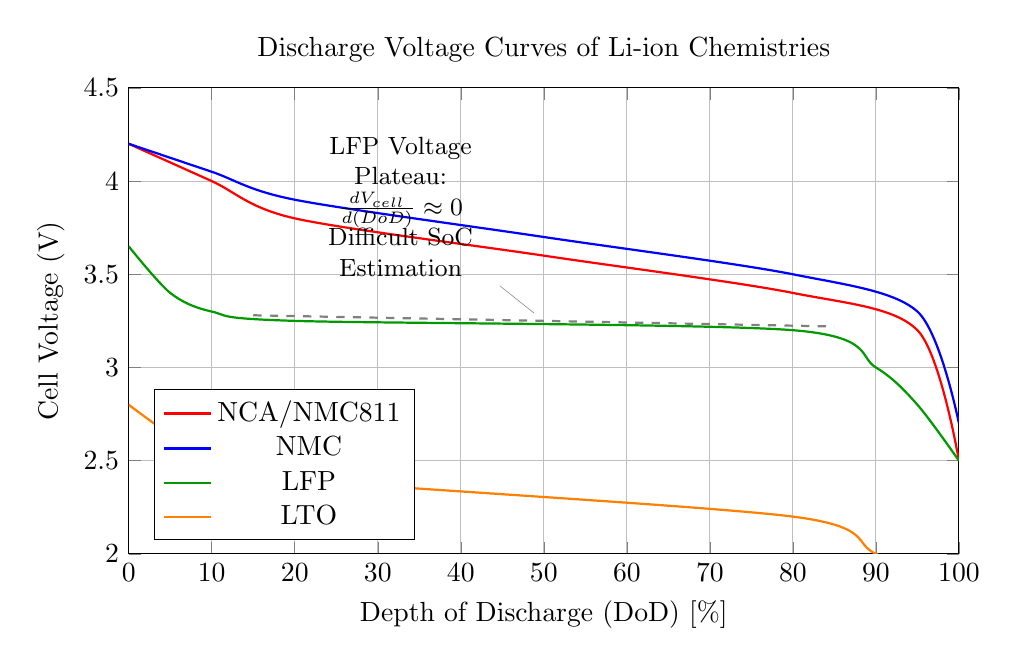
\begin{tikzpicture}
        \begin{axis}[
            title={Discharge Voltage Curves of Li-ion Chemistries},
            xlabel={Depth of Discharge (DoD) [\%]},
            ylabel={Cell Voltage (V)},
            xmin=0, xmax=100,
            ymin=2.0, ymax=4.5,
            grid=major,
            legend pos=south west,
            width=\textwidth,
            height=7.5cm,
        ]
        \addplot[smooth, thick, red] coordinates { (0, 4.2) (10, 4.0) (20, 3.8) (50, 3.6) (80, 3.4) (95, 3.2) (100, 2.5) };
        \addlegendentry{NCA/NMC811}

        \addplot[smooth, thick, blue] coordinates { (0, 4.2) (10, 4.05) (20, 3.9) (50, 3.7) (80, 3.5) (95, 3.3) (100, 2.7) };
        \addlegendentry{NMC}

        \addplot[smooth, thick, green!60!black] coordinates { (0, 3.65) (5, 3.4) (10, 3.3) (20, 3.25) (80, 3.2) (90, 3.0) (95, 2.8) (100, 2.5) };
        \addlegendentry{LFP}
        
        \addplot[smooth, thick, orange] coordinates { (0, 2.8) (10, 2.5) (20, 2.4) (80, 2.2) (90, 2.0) (100, 1.8) };
        \addlegendentry{LTO}

        \draw[dashed, thick, gray] (axis cs:15,3.28) -- (axis cs:85,3.22);
        \node[pin=135:{\parbox{2.5cm}{\centering \small LFP Voltage Plateau: \\ $\frac{dV_{cell}}{d(DoD)} \approx 0$ \\ Difficult SoC Estimation}}] at (axis cs:50,3.25) {};
        \end{axis}
    \end{tikzpicture}
    \caption{Typical discharge voltage curves for various lithium-ion chemistries. The extremely flat profile of LFP makes accurate SoC estimation challenging based on voltage alone, necessitating more complex estimation techniques like Coulomb counting and periodic recalibration\footcite{plett2015battery}.}
    \label{fig:voltage_curves_detailed}
\end{figure}
\noindent
As shown in Figure \ref{fig:voltage_curves_detailed}, LFP's remarkably flat voltage plateau makes it nearly impossible for BMS to determine precise SoC in the central operating range (from approximately 20\% to 80\%) using voltage alone. This necessitates more complex estimation techniques, such as Coulomb counting (integrating current over time), which can suffer from drift. To correct this drift, LFP-equipped vehicles require periodic full charges to 100\% for BMS recalibration. This represents an important operational constraint that V2G control strategies must consider.

\subsection{Comparative Analysis and Safety Considerations}

The trade-offs between chemistries are summarized in Table \ref{tab:chem_comparison_detailed}. Safety remains paramount, with the primary risk being thermal runaway—a dangerous, self-sustaining exothermic reaction. This risk relates directly to cathode material chemical and thermal stability. Higher energy density generally means more energy packed into smaller mass, which can be released violently if cells are compromised. Consequently, critical temperatures for initiating thermal runaway are generally lower for higher energy density chemistries. LFP's stable phosphate-based structure makes it far more resistant to thermal runaway than nickel-based counterparts, a key reason for its growing popularity.

\begin{table}[h!]
\centering
\small
\caption{Comparative analysis of key automotive battery chemistries, highlighting the trade-offs between performance and safety.}
\label{tab:chem_comparison_detailed}
\begin{tabularx}{\textwidth}{
  @{}
  >{\bfseries\RaggedRight}X
  *{5}{C}
  @{}
}
\toprule
Metric & NCA & NMC & LFP & LTO & LCO \\
\midrule
Energy Density (Wh/kg) & 200 - 260 (Highest) & 150 - 220 (High) & 90 - 160 (Moderate) & 60 - 110 (Low) & 150-200 (High) \\
\addlinespace
Cycle Life & 1000 - 2000 & 1000 - 2500 & 2000 - 5000+ & $>$10,000 & 500 - 1000 \\
\addlinespace
Safety & Good & Very Good & Excellent & Excellent & Poor \\
\addlinespace
Thermal Runaway Temp ($^{\circ}$C) & $\sim$150 - 180 & $\sim$180 - 210 & $\sim$220 - 270 & $>$ 250 & $\sim$150 \\
\bottomrule
\end{tabularx}
\end{table}